\chapter{Appendix for Structural Changes in Doped and Excited Conjugated Polymers}

\section{Polythiophene Torsion Potentials}
\label{sec:pt_tp}
\subsection{Torsion Potential Data and Initial Structures}
\
\\[1.5in]
\begin{table}[hbt!]\centering
\caption{Ground-state Thiophene Dimer Initial Structure}
\renewcommand{\arraystretch}{1.5}
\begin{threeparttable}
\begin{tabular}{ccccc}\toprule
{} & {Atom} & {X (\AA)} & {Y (\AA)} & {Z (\AA)} \\ \midrule
  1 & S & -0.0023723 & -0.0560977 & -0.0300969\\
  2 & C & 1.7070035 & -0.0292241 & -0.0145267\\
  3 & H & 2.2421009 & -0.0503556 & 0.9188681\\
  4 & C & 2.2188238 & 0.0166957 & -1.2731976\\ \midrule
  5 & H & 3.2760435 & 0.0396095 & -1.4857363\\
  6 & C & 1.2080458 & 0.0437755 & -2.2700460\\
  7 & H & 1.4022626 & 0.1035054 & -3.3303301\\
  8 & C & -0.0534481 & 0.0159971 & -1.7485209\\ \midrule
  9 & C & -1.3283732 & 0.0357503 & -2.4552048\\
  10 & C & -2.5140867 & 0.5793303 & -2.0518483\\
  11 & H & -2.6304470 & 1.0993723 & -1.1131149\\
  12 & C & -3.5508397 & 0.4152358 & -3.0079307\\ \midrule
  13 & H & -4.5565336 & 0.7819288 & -2.8760054\\
  14 & C & -3.1332923 & -0.2472315 & -4.1192789\\
  15 & H & -3.7048930 & -0.4997928 & -4.9952883\\
  16 & S & -1.4859744 & -0.6908589 & -4.0068121\\ \bottomrule
\end{tabular}
\begin{tablenotes}
\item
\end{tablenotes}
\end{threeparttable}
\end{table}

\begin{table}[hbt!]\centering
\caption{Ground-state Thiophene Dimer Torsion Data}
\renewcommand{\arraystretch}{1.5}
\begin{threeparttable}
\begin{tabular}{cccc}\toprule
  {} & {Torsion Angle} & {Rel. Energy (eV)} & {Abs. Energy (Hartree)} \\ \midrule
    1 & 0.0 & 0.04598 & -1104.84987203842\\
    2 & 10.0 & 0.03979 & -1104.85009939477\\
    3 & 20.0 & 0.02779 & -1104.85054035879\\
    4 & 30.0 & 0.01928 & -1104.85085335093\\ \midrule
    5 & 40.0 & 0.01868 & -1104.85087543253\\
    6 & 50.0 & 0.02689 & -1104.85057349252\\
    7 & 60.0 & 0.04200  & -1104.85001836446\\
    8 & 70.0 & 0.05898 & -1104.84939439490\\ \midrule
    9 & 80.0 & 0.07241 & -1104.84890093182\\
    10 & 90.0 & 0.07646 & -1104.84875201328\\
    11 & 100.0 & 0.06924 & -1104.84901713984\\
    12 & 110.0 & 0.05278 & -1104.84962222807\\ \midrule
    13 & 120.0 & 0.03288 & -1104.85035334414\\
    14 & 130.0 & 0.01530 & -1104.85099955470\\
    15 & 140.0 & 0.00358 & -1104.85143006908\\
    16 & 150.0 & 0.00000 & -1104.85156180070\\ \midrule
    17 & 160.0 & 0.00326 & -1104.85144196165\\
    18 & 170.0 & 0.00927 & -1104.85122115615\\
    19 & 180.0 & 0.01234 & -1104.85110839823\\ \bottomrule
\end{tabular}
\begin{tablenotes}
\item
\end{tablenotes}
\end{threeparttable}
\end{table}

\begin{table}[hbt!]\centering
\caption{Doped-state Thiophene Dimer Initial Structure}
\renewcommand{\arraystretch}{1.5}
\begin{threeparttable}
\begin{tabular}{ccccc}\toprule
{} & {Atom} & {X (\AA)} & {Y (\AA)} & {Z (\AA)} \\ \midrule
  1 & S & 0.0003979 & 0.4373270 & -0.0633642\\
  2 & C & 1.6743230 & 0.2163099 & -0.0571461\\
  3 & H & 2.2287328 & 0.3339913 & 0.8611866\\
  4 & C & 2.1929799 & -0.1115590 & -1.3041171\\ \midrule
  5 & H & 3.2426659 & -0.2866798 & -1.4795321\\
  6 & C & 1.2098407 & -0.1839581 & -2.2716885\\
  7 & H & 1.3925319 & -0.4251174 & -3.3088107\\
  8 & C & -0.0772964 & 0.0912069 & -1.7653271\\ \midrule
  9 & C & -1.2859459 & 0.1035335 & -2.4670641\\
  10 & C & -2.5730754 & 0.3787571 & -1.9607149\\
  11 & H & -2.7557610 & 0.6199609 & -0.9236020\\
  12 & C & -3.5562300 & 0.3062435 & -2.9282622\\ \midrule
  13 & H & -4.6059215 & 0.4813222 & -2.7528378\\
  14 & C & -3.0375815 & -0.0216838 & -4.1752213\\
  15 & H & -3.5920046 & -0.1394621 & -5.0935336\\
  16 & S & -1.3636358 & -0.2425520 & -4.1690348\\ \bottomrule
\end{tabular}
\begin{tablenotes}
\item
\end{tablenotes}
\end{threeparttable}
\end{table}

\begin{table}[hbt!]\centering
\caption{Doped-state Thiophene Dimer Torsion Data}
\renewcommand{\arraystretch}{1.5}
\begin{threeparttable}
\begin{tabular}{cccc}\toprule
  {} & {Torsion Angle} & {Rel. Energy (eV)} & {Abs. Energy (Hartree)} \\ \midrule
    1 & 0.0 & 0.02079 & -1104.50938633204\\
    2 & 10.0 & 0.02825 & -1104.50911231215\\
    3 & 20.0 & 0.05223 & -1104.50823104848\\
    4 & 30.0 & 0.09371 & -1104.50670665615\\ \midrule
    5 & 40.0 & 0.15812 & -1104.50433961960\\
    6 & 50.0 & 0.24644 & -1104.50109374877\\
    7 & 60.0 & 0.35673 & -1104.49704060708\\
    8 & 70.0 & 0.48820 & -1104.49220922909\\ \midrule
    9 & 80.0 & 0.63920 & -1104.48666033352\\
    10 & 90.0 & 0.78498 & -1104.48130300611\\
    11 & 100.0 & 0.62139 & -1104.48731456600\\
    12 & 110.0 & 0.47554 & -1104.49267465589\\ \midrule
    13 & 120.0 & 0.34797 & -1104.49736261553\\
    14 & 130.0 & 0.24010 & -1104.50132673110\\
    15 & 140.0 & 0.15423 & -1104.50448240244\\
    16 & 150.0 & 0.08729 & -1104.50694235511\\ \midrule
    17 & 160.0 & 0.03966 & -1104.50869281167\\
    18 & 170.0 & 0.01087 & -1104.50975071487\\
    19 & 180.0 & 0.00000 & -1104.51015031856\\ \bottomrule
\end{tabular}
\begin{tablenotes}
\item
\end{tablenotes}
\end{threeparttable}
\end{table}

\begin{table}[hbt!]\centering
\caption{Excited-state Thiophene Dimer Initial Structure}
\renewcommand{\arraystretch}{1.5}
\begin{threeparttable}
\begin{tabular}{ccccc}\toprule
{} & {Atom} & {X (\AA)} & {Y (\AA)} & {Z (\AA)} \\ \midrule
  1 & S & -0.0180675 & 0.4466192 & -0.0408593\\
  2 & C & 1.6926804 & 0.2166109 & -0.0439241\\
  3 & H & 2.2550459 & 0.3305548 & 0.8671136\\
  4 & C & 2.1935848 & -0.1115653 & -1.3030670\\ \midrule
  5 & H & 3.2449313 & -0.2870510 & -1.4774923\\
  6 & C & 1.2341910 & -0.1883271 & -2.2796908\\
  7 & H & 1.4178092 & -0.4288461 & -3.3154027\\
  8 & C & -0.1008011 & 0.0925904 & -1.7763147\\ \midrule
  9 & C & -1.2624454 & 0.1021336 & -2.4560715\\
  10 & C & -2.5974302 & 0.3830769 & -1.9527024\\
  11 & H & -2.7810468 & 0.6236319 & -0.9169985\\
  12 & C & -3.5568312 & 0.3062823 & -2.9293227\\ \midrule
  13 & H & -4.6081778 & 0.4817637 & -2.7548939\\
  14 & C & -3.0559380 & -0.0219757 & -4.1884438\\
  15 & H & -3.6183064 & -0.1359654 & -5.0994740\\
  16 & S & -1.3451782 & -0.2518931 & -4.1915259\\ \bottomrule
\end{tabular}
\begin{tablenotes}
\item
\end{tablenotes}
\end{threeparttable}
\end{table}

\begin{table}[hbt!]\centering
\caption{Excited-state Thiophene Dimer Torsion Data}
\renewcommand{\arraystretch}{1.5}
\begin{threeparttable}
\begin{tabular}{cccc}\toprule
  {} & {Torsion Angle} & {Rel. Energy (eV)} & {Abs. Energy (Hartree)} \\ \midrule
    1 & 0.0 & 0.01269 & -1104.69509558720\\
    2 & 10.0 & 0.02498 & -1104.69464387418\\
    3 & 20.0 & 0.06486 & -1104.69317837941\\
    4 & 30.0 & 0.13225 & -1104.69070196155\\ \midrule
    5 & 40.0 & 0.22992 & -1104.68711247641\\
    6 & 50.0 & 0.36069 & -1104.68230686926\\
    7 & 60.0 & 0.50986 & -1104.67682512101\\
    8 & 70.0 & 0.64448 & -1104.67187782963\\ \midrule
    9 & 80.0 & 0.75853 & -1104.66768637840\\
    10 & 90.0 & 0.84183 &  -1104.66462531896\\
    11 & 100.0 & 0.76183 & -1104.66756522231\\
    12 & 110.0 & 0.65961 & -1104.67132193500\\ \midrule
    13 & 120.0 & 0.53077 & -1104.67605665532\\
    14 & 130.0 & 0.38036 & -1104.68158410041\\
    15 & 140.0 & 0.24551 & -1104.68653968278\\
    16 & 150.0 & 0.13895 & -1104.69045559904\\ \midrule
    17 & 160.0 & 0.06376 & -1104.69321900264\\
    18 & 170.0 & 0.01692 & -1104.69494025977\\
    19 & 180.0 & 0.00000 & -1104.69556201328\\ \bottomrule
\end{tabular}
\begin{tablenotes}
\item
\end{tablenotes}
\end{threeparttable}
\end{table}

\clearpage
\subsection{Ground-state Torsion Potentials at Different Levels of Theory}
\
\begin{figure}[hbt!]
    \centering
    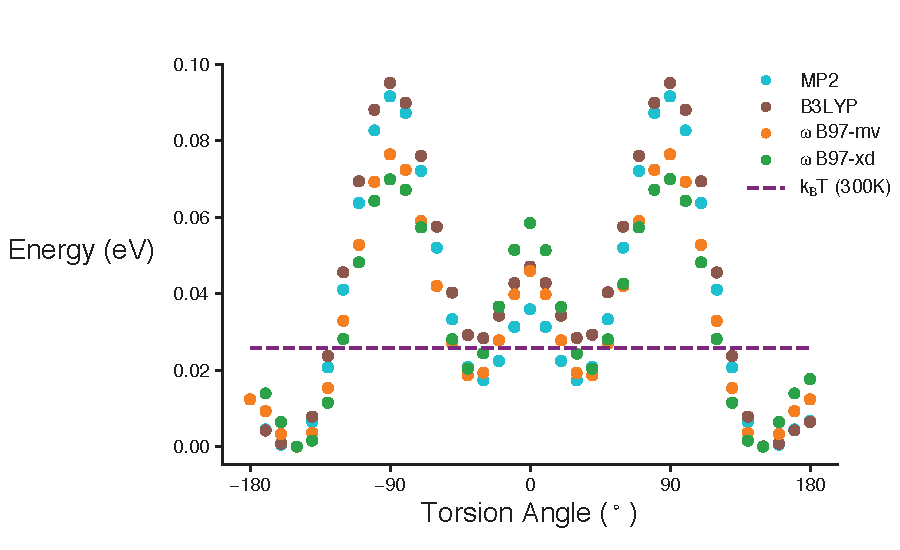
\includegraphics{figures/append_tor_model/SI_compare_theory_torsion.pdf}
    \caption{Ground-state torsion potential at different levels of theory. MP2 basis set: cc-pVTZ, B3LYP and $\omega$B97-xd basis set: 6-31++G**, $\omega$B97-mv basis set: def2-QZVPPD}
    \label{fig:gs_theory}
\end{figure}

\subsection{The Effect of Chain Length on Ground-state Torsion Angles}
\label{subsec:chain_length_gs}

Different polythiophene (PT) chain lengths were optimized at the RI-MP2 level (Figure \ref{tab:gs_RIMP2}). In all instances the optimized structures had non-planar central torsion angles corresponding to minima observed in Figure \ref{fig:gs_theory}. Additionally, the energy of optimized planar (trans) configurations were higher than that of optimized non-planar configurations. This evidence supports DuBay et al. in their claim that the torsion potential of conjugated polymers such as PT can be approximated by the dimer torsion potential if an appropriate level of theory, basis set, and optimization procedure are used.\cite{Dubay2012}

\begin{table}[hbt!]\centering
\caption{Ground-state Optimized Geometries}
\label{tab:gs_RIMP2}
\renewcommand{\arraystretch}{1.5}
\begin{threeparttable}
\begin{tabular}{cccc}\toprule
\multicolumn{1}{c}{\multirow{2}{2.5cm}{\centering Number of \\ Monomers}} &
\multicolumn{1}{c}{\multirow{2}{4.1cm}{\centering Trans Geometry \\ Abs. Energy (Hartree)}} &
\multicolumn{1}{c}{\multirow{2}{4.1cm}{\centering Optimized Geometry \\ Abs. Energy (Hartree)}} &
\multicolumn{1}{c}{\multirow{2}{4.1cm}{\centering Optimized Central  \\ Torsion Angle ($^\circ$)}} \\ \\ \midrule
    2 & -1103.35246329362\tnote{a} & -1103.35284395916\tnote{a} & 22\\
    4 & -2205.26456300358\tnote{b} & -2205.26519616574\tnote{b} & 161\\
    8 & -- & -4409.36496730408\tnote{b} & 159\\ \bottomrule
\end{tabular}
\begin{tablenotes}
\item[a] \footnotesize Theory: RI-MP2 basis set: cc-pVQZ
\item[b] \footnotesize Theroy: RI-MP2 basis set: cc-pVTZ
\end{tablenotes}
\end{threeparttable}
\end{table}

\clearpage
